\setcounter{figure}{0}

\section{22nd October 2023: I AM the door of the sheep, I AM the good Shepherd}
\subsection*{Text: John 10:1-21}
  \begin{quote}
  [1] “Truly, truly, I say to you, he who does not enter the sheepfold by the door but climbs in by another way, that man is a thief and a robber. [2] But he who enters by the door is the shepherd of the sheep. [3] To him the gatekeeper opens. The sheep hear his voice, and he calls his own sheep by name and leads them out. [4] When he has brought out all his own, he goes before them, and the sheep follow him, for they know his voice. [5] A stranger they will not follow, but they will flee from him, for they do not know the voice of strangers.” [6] This figure of speech Jesus used with them, but they did not understand what he was saying to them.

  [7] So Jesus again said to them, “Truly, truly, I say to you, I am the door of the sheep. [8] All who came before me are thieves and robbers, but the sheep did not listen to them. [9] I am the door. If anyone enters by me, he will be saved and will go in and out and find pasture. [10] The thief comes only to steal and kill and destroy. I came that they may have life and have it abundantly. [11] I am the good shepherd. The good shepherd lays down his life for the sheep. [12] He who is a hired hand and not a shepherd, who does not own the sheep, sees the wolf coming and leaves the sheep and flees, and the wolf snatches them and scatters them. [13] He flees because he is a hired hand and cares nothing for the sheep. [14] I am the good shepherd. I know my own and my own know me, [15] just as the Father knows me and I know the Father; and I lay down my life for the sheep. [16] And I have other sheep that are not of this fold. I must bring them also, and they will listen to my voice. So there will be one flock, one shepherd. [17] For this reason the Father loves me, because I lay down my life that I may take it up again. [18] No one takes it from me, but I lay it down of my own accord. I have authority to lay it down, and I have authority to take it up again. This charge I have received from my Father.”

  [19] There was again a division among the Jews because of these words. [20] Many of them said, “He has a demon, and is insane; why listen to him?” [21] Others said, “These are not the words of one who is oppressed by a demon. Can a demon open the eyes of the blind?”
  \end{quote}
\subsection*{Notes}
\begin{itemize}
  \item{Recap: “I AM” (Ego Eimi) is the covenant name of God in the OT. The 7 “I AM” statements is Jesus making a declaration about himself. The response to Jesus’ declaration of his identity is very varied, see v19-21. Even today, Jesus invites us to respond to this declaration of His identity, as the divine Son of God. There is usually a context to Jesus’ “I AM” statements. “I AM the bread of life” has the passover has the context, “I AM the light of the world” has the feast of booths as the context.} 
  \item{Immediately after the light of the world, there is the healing of the blind man. This was especially significant, cause Jesus now gives the blind man light. The healing of the blind man also precedes the “I AM the door” and “I AM the good shepherd” discourse. This is because after the blind man was healed, the Pharisees were unhappy, because the healing happened on a Sabbath. This is an example of the Pharisees oppressing God’s people.}
  \item{Hence, in today’s text we see that Jesus is contrasting himself with the pharisees. The pharisees are the bad shepherds, they are the hired hand, they are the thief and robber. Whereas, Jesus is the door and thr good shepherd. }
  \item{And we are being compared with sheep. Sheep are very defenceless, timid and helpless animals. Without the shepherd, the sheep will do stupid stuff. And when the sheep rolls over on its back, it can’t help itself, the shepherd needs to roll the sheep over. This is us, we are utterly helpless. And each of us like sheep has gone astray :(. But this is where Jesus comes in…}
  \item{First point: Jesus knows his sheep intimately. Jesus calls his sheep by name, and his sheep know Jesus, and they know his voice. So for us, we know that Jesus knows us very well. He knows all of our weaknesses, our characteristics, and all the help we need. And for us, we know that we need to respond to Jesus voice, and we need to ignore the voices of strangers (the ways of the world).}
  \item{Second point: a good shepherd protects and provides for his sheep. There are some makeshift sheep pens where the shepherd lies down as the door, to protect the sheep from wolves. This way, we are safe from our enemies, we don’t need to worry, because there is our good shepherd who is the door that protects us. And here, we see that Jesus is the only way to salvation. Only through Jesus can we find pasture and life everlasting. }
  \item{Third point: the good shepherd lays down his life for his sheep. When predators like bears and wolves come, the shepherd needs to fight the sheep. But one thing to note here is that the shepherd lays down his life willingly and lovingly and obediently to the Father. This is a metaphor to what Jesus does for us on the cross. Jesus gave his life for us, to save us from sin and the power of the devil, to make us just and to give us a new heart. And we see here that Jesus also has authority to take up his life again. A normal shepherd lays down his life for the sheep to fend off invaders, but after dying, his sheep become helpless from other invaders. Here, Jesus lays down his life for his sheep willingly on the cross, but he also takes up his life again to intercede for us before the Father, keeping us safe perpetually.}
  \item{Why is Jesus the only way? This is because Christianity is the only religion that says that our creator took on human flesh, entered our filthy world, and died on the cross for us, and was raised up for us. Other religions tells us to “do things and be saved”, Christianity is the only religion that says “all things are done for you”. And we enter through Jesus by faith alone. When we enter into a relationship with God through Jesus, not only are we saved (from sin), we are also safe and secure, being in the sheep pen (safe from the devil and from sin). And we have full satisfaction (r/s with God satisfies us fully), since Jesus gives us pasture.}
  \item{And for us, as mentioned above, we need to learn how to hear Jesus’ voice better and better, and to ignore the world’s voice more and more. We need to better know our Shepherd. And as a result, we can better trust our shepherd. Even if our shepherd seems to lead us to seemingly strange and dark places, we know that it is for our good, because our shepherd is a good shepherd. }
  % \item{\begin{figure}[H]
  %   \centering
  %   % 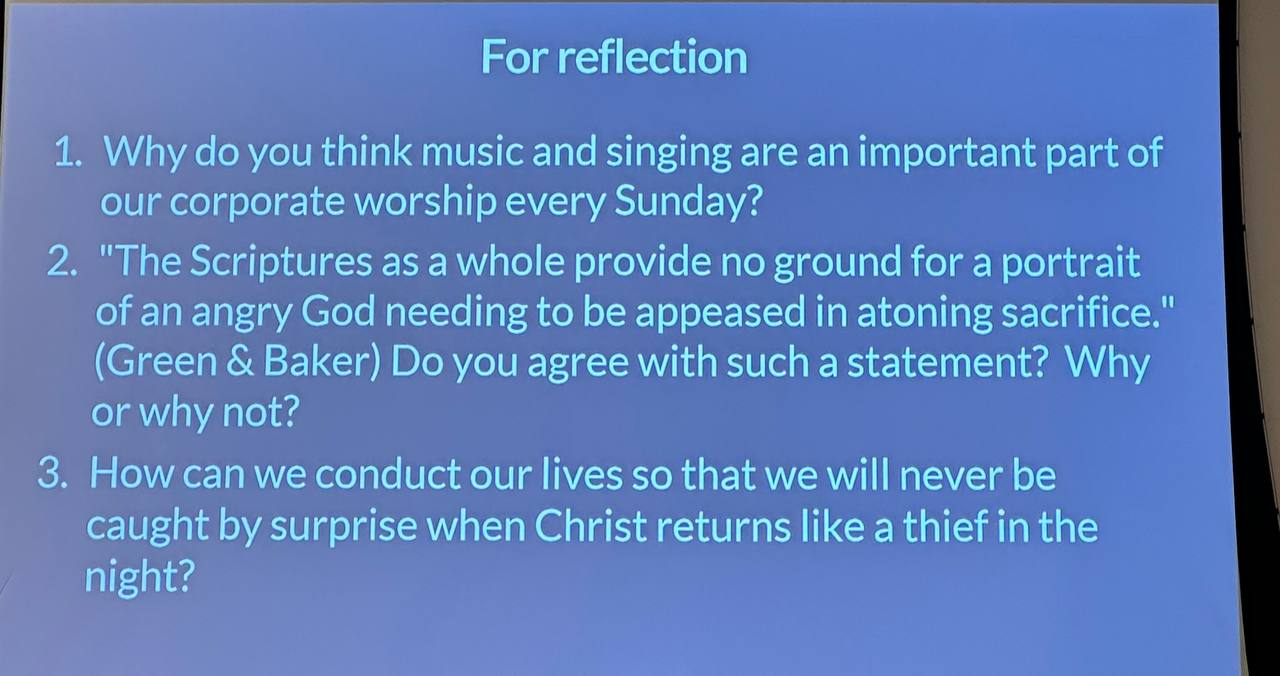
\includegraphics[width=0.8\textwidth, trim={0cm 0cm 0cm 0cm},clip]{Figures/marchSermon4Reflections.jpg}
  %   \includegraphics[width=0.8\textwidth, trim={0cm 0cm 0cm 0cm},clip]{example-image-a}
  %   \caption[]{Reflection questions for this sermon}
  %   \label{}
  % \end{figure}}
\end{itemize}